% !TeX spellcheck = fr_FR
\documentclass[a4paper, 11pt]{report}


%% Language and font encodings
\usepackage[french]{babel}
\usepackage[utf8]{inputenc}
\usepackage[T1]{fontenc}

%% Sets page size and margins
\usepackage[a4paper,top=3cm,bottom=2cm,left=2.5cm,right=2.5cm,marginparwidth=1.75cm]{geometry}

%% Useful packages
\usepackage{biblatex}
\bibliography{report.bib}
\usepackage{graphicx}
\usepackage[colorinlistoftodos]{todonotes}
\usepackage{amsmath,amsthm,amssymb}
\usepackage[colorlinks=true, allcolors=blue]{hyperref}
\usepackage{listings}
\usepackage{color}
\usepackage{titlesec}
\definecolor{dkgreen}{rgb}{0,0.6,0}
\usepackage{textcomp}
\lstset{frame=tb,
  language=Python,
  aboveskip=3mm,
  belowskip=3mm,
  showstringspaces=false,
  columns=flexible,
  basicstyle={\ttfamily},
  numbers=none,
  numberstyle=\color{gray},
  keywordstyle=\color{blue},
  commentstyle=\color{dkgreen},
  stringstyle=\color{dkgreen},
  breaklines=true,
  breakatwhitespace=true,
  tabsize=2
}
\setlength{\parskip}{1em}

\titleformat{\chapter}{\normalfont\huge}{\bf\thechapter}{12pt}{\huge\bf}

\title{TB - Gleam}

\author{Antoine Friant}
\pagenumbering{roman}
\begin{document}
\begin{titlepage}

\newcommand{\HRule}{\rule{\linewidth}{0.5mm}} % Defines a new command for the horizontal lines, change thickness here
%----------------------------------------------------------------------------------------
%	LOGO SECTION
%----------------------------------------------------------------------------------------


\includegraphics[width=2in]{img/logoheig.png}\\ % Include a department/university logo - this will require the graphicx package

\vspace{1in}

\center % Center everything on the page
 
%----------------------------------------------------------------------------------------
%	HEADING SECTIONS
%----------------------------------------------------------------------------------------

\textsc{\LARGE HEIG-VD}\\[1.5cm] % Name of your university/college
\textsc{\Large Rapport intermédiaire}\\[0.5cm] % Major heading such as course name

%----------------------------------------------------------------------------------------
%	TITLE SECTION
%----------------------------------------------------------------------------------------

\HRule \\[0.4cm]
{ \huge \bfseries La Terre de nuit vue de l'espace }\\ % Title of your document
\Large\HRule \\[2cm]
\normalsize
%----------------------------------------------------------------------------------------
%	AUTHOR SECTION
%----------------------------------------------------------------------------------------

\begin{minipage}[t]{0.48\textwidth}
\begin{flushleft} \large
Antoine \textsc{Friant} \\
\normalsize
Haute École d'Ingénierie et de Gestion du Canton de Vaud\\
Yverdon-les-Bains, VD, CH
\texttt{antoine.friant@gmail.com}
\end{flushleft}
\end{minipage}
~
\begin{minipage}[t]{0.49\textwidth}
\begin{flushright} \large
% empty page for alignement
\end{flushright}
\end{minipage}\\[2cm]



{\large \today}\\
 

\vfill % Fill the rest of the page with whitespace

\end{titlepage}

\tableofcontents

\chapter{Cahier des charges}

\section{Résumé du problème}
Les données géographiques sont nécessaires pour la prise de décisions importantes. Cependant la fiabilité et la disponibilité de ces données ne sont pas homogènes dans le temps et selon le lieu. Certaines de ces données ont une forte corrélation avec la lumière perçue par les satellites pendant la nuit.

Grâce à l'apprentissage automatique (\textit{machine learning}), il est possible d'entraîner un réseau de neurones sur des données d'une date et d'un lieu connus pour reconstituer une carte de données géographiques à partir d'une image satellite nocturne.

Le travail à effectuer consiste à explorer différents types de données géographiques afin d'en choisir un, et faire de la prédiction sur ce type de données grâce à un réseau de neurones.

\section{Objectifs}
Le TB consiste dans un premier temps à explorer les données suivantes :

\begin{itemize}
\item Images satellites noctures de la Terre,
\item Population humaine,
\item Population animale,
\item Densité végétale,
\item PIB,
\end{itemize}

Et toutes autres données jugées pertinentes dans le but d'entraîner un réseau de neurones capable de prédire une estimation d'une donnée utile, à partir d'une image satellite de la terre de nuit.

La réalisation d'une application qui entraîne et exploite ce réseau de neurones est l'objectif de la seconde partie du TB.

Le but final est de pouvoir estimer, grâce au machine learning, des informations dont on ne possède pas de données à jour. Et cela à partir d'images satellites de nuit récentes, ou d'une combinaison de ces images avec une autre donnée à jour.

\section{Limitations}
L'application sera compatible avec Windows 10 et Archlinux, et nécessitera l'installation de librairies tierces (telles que Keras et TensorFlow).
Elle ne possèdera pas nécessairement d'interface utilisateur.

L'utilisateur sera responsable de fournir les données à l'application dans un format supporté.

\section{Description fonctionnelle}
L'application prend en argument au moins deux jeux de données géographiques de format imposé : une image satellite nocturne et un autre type de donnée à déterminer au cours du projet. Après un long temps d'entraînement (une semaine au maximum, dépend de la machine utilisée), un modèle est généré.

Une fois le modèle généré, il est sauvegardé et réutilisable sur une autre image satellite nocturne (d'une date et/ou d'une région différente). Lorsque le modèle est appliqué sur une image satellite, une carte est recréée, affichant le résultats des prédictions.

Par exemple, si au cours du travail de bachelor il s'avère que la population par kilomètre carré est une donnée utile et utilisable, l'application devra prendre en argument une image satellite nocturne ainsi qu'une carte des populations de même taille et de même résolution pour entraîner le réseau de neurones. Une fois le modèle généré, l'application devra être capable de regénéré une approximation de la carte de population par kilomètre carré à partir d'une image satellite.

\section{Délais}
\textbf{15 juin 2018 :} Rapport intermédiaire

\textbf{27 juillet 2018 :} Rapport final et application fonctionnelle

\textbf{Entre le 3 et le 14 septembre 2018 :} Soutenance du travail de bachelor

%\chapter{Résumé}


\chapter{Introduction}
\pagenumbering{arabic}
Les produits d'imagerie satellite sont devenus abondants et largement accessible au cours des dernières décennies. De nombreux satellites prennent des photographies de la Terre à chaque heure du jour \textit{et de la nuit}. Les observations nocturnes révèlent des caractéristiques peu évidentes de jour, parfois même cachées. Les routes apparaissent, les villes montrent leurs lumières, même les bateaux de pêche aveuglent les océans avec des projecteurs pour attirer les poissons.

La disponibilité, la résolution et l'uniformité de la qualité de ces données contraste fortement avec le manque de fiabilité d'autres informations géographiques utiles lors de prises de décisions importantes. Par exemple, la densité de la population est une estimation précise en Suisse mais très approximative au Kenya. D'autres mesures intéressantes incluent : la consommation en électricité, les émissions de C0$_2$, la couverture végétale et la présence de faune. Les lumières nocturnes observées depuis l'espace donnent des indications sur chacune de ces mesures alors qu'elles peuvent manquer dans une région à une date donnée.

Le but de ce projet est d'extraire autant d'information que possible de l'imagerie satellite nocturne en utilisant l'apprentissage automatique (\textit{machine learning}) sous la forme dê réseau de neurones.

\chapter{Exploration des données}
\section{Jeux de données}
\subsection{Images satellite}
\subsubsection{NASA Worldview}
La première source de données explorée est l'application "Worldview" de la NASA \cite{nasa-worldview}. Elle permet de visionner un grand nombre d'images satellite composites sur un globe en trois dimensions (voir figure \ref{nasa-worldview-screenshot}). Parmi les jeu de données disponibles sont trois jeux d'images nocturnes.

\begin{figure}[h]
	\centering
	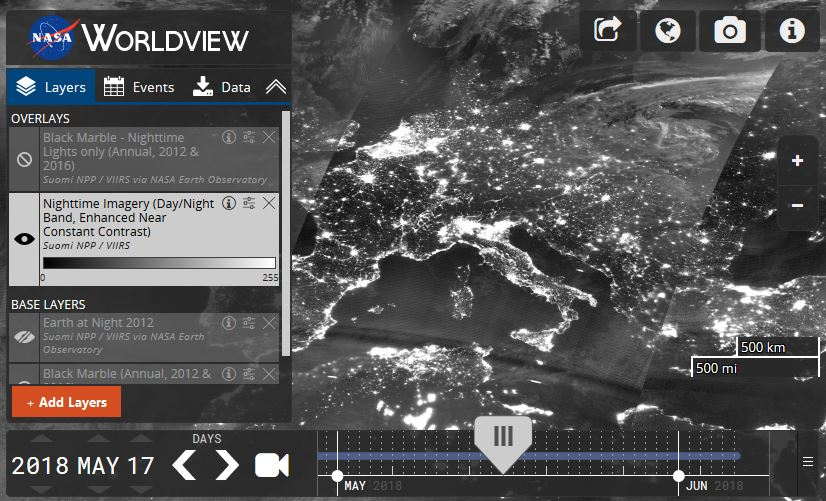
\includegraphics[width=1.0\textwidth]{img/worldview.JPG}
	\caption{Outil de visualisation NASA Worldview \cite{nasa-worldview}.}
	\label{nasa-worldview-screenshot}
\end{figure}

Le premier jeu de données est série d'images composites capturées par le satellite Suomi NPP opéré par la NASA, la NOAA et le Département de la Défense des États-Unis. Il est mis à jour toutes les quelques heures, et présente une image composite chaque jour depuis le 30 novembre 2016. Elle possède deux défauts éliminatoires : la période d'observation actuellement disponible (à peine plus d'une année) n'est pas suffisamment longue pour observer une évolution significative des villes depuis l'espace, et les images ne sont pas traitées. Cela signifie que celles-ci sont très fortement bruitées par les nuages et la lumière ambiante due aux différentes phases de la Lune.

\begin{figure}[h]
	\centering
	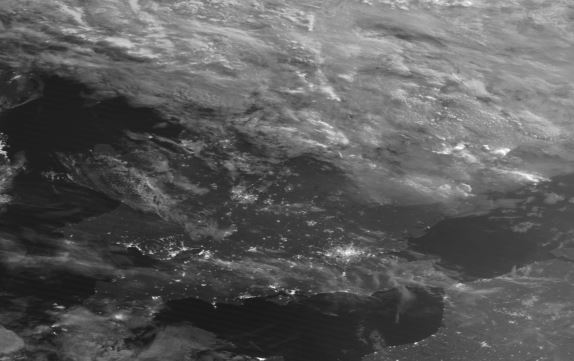
\includegraphics[width=0.5\textwidth]{img/worldview_clouds.JPG}
	\caption{Image satellite quotidienne servie par NASA Worldview \cite{nasa-worldview}, représentant la Grande Bretagne et son climat nuageux.}
	\label{nasa-worldview-daily}
\end{figure}

Les deux autres jeux de données nocturnes sont des images composites : des clichés pris tout au long de l'année ont permis de fabriquer une seule image du globe dont la luminosité ambiante est constante (moyennée) et sur laquelle les nuages n'apparaissent pas. Malheureusement, l'outil Worldview ne permet pas un téléchargement direct de ces images \textit{dans leur pleine résolution}. Heureusement, la NASA a mis à disposition une API REST (\url{https://wiki.earthdata.nasa.gov/display/GIBS/GIBS+API+for+Developers}) pour télécharger des "tuiles" de n'importe laquelle de leur image. Seulement le format PNG est disponible. Ce format ne contient pas d'information géographiques, ce qui complique leur utilisation pour la suite de ce travail. Un script Python suffit pour télécharger et assembler les tuiles (figure \ref{nasa-worldview-tile}) pour reconstituer une image complète du globe de plus de 800 millions de pixels (figure \ref{nasa-worldview-tiles}).

\begin{figure}[h]
	\centering
	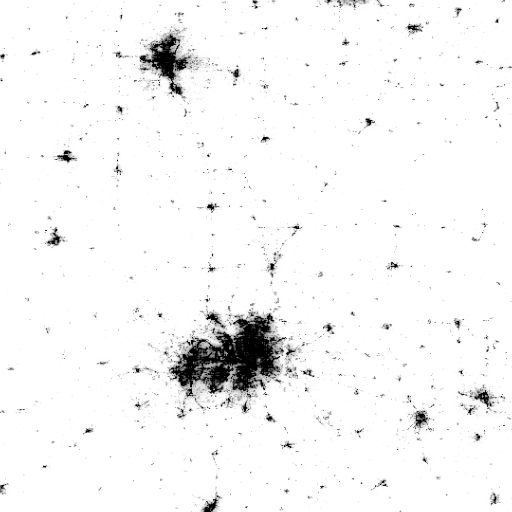
\includegraphics[width=0.5\textwidth]{img/018-012.png}
	\caption{Une tuile de l'image de 2016 montrant la ville de Dallas (USA) après avoir été mise en couleurs négatives.}
	\label{nasa-worldview-tile}
\end{figure}

\begin{figure}
	\centering
	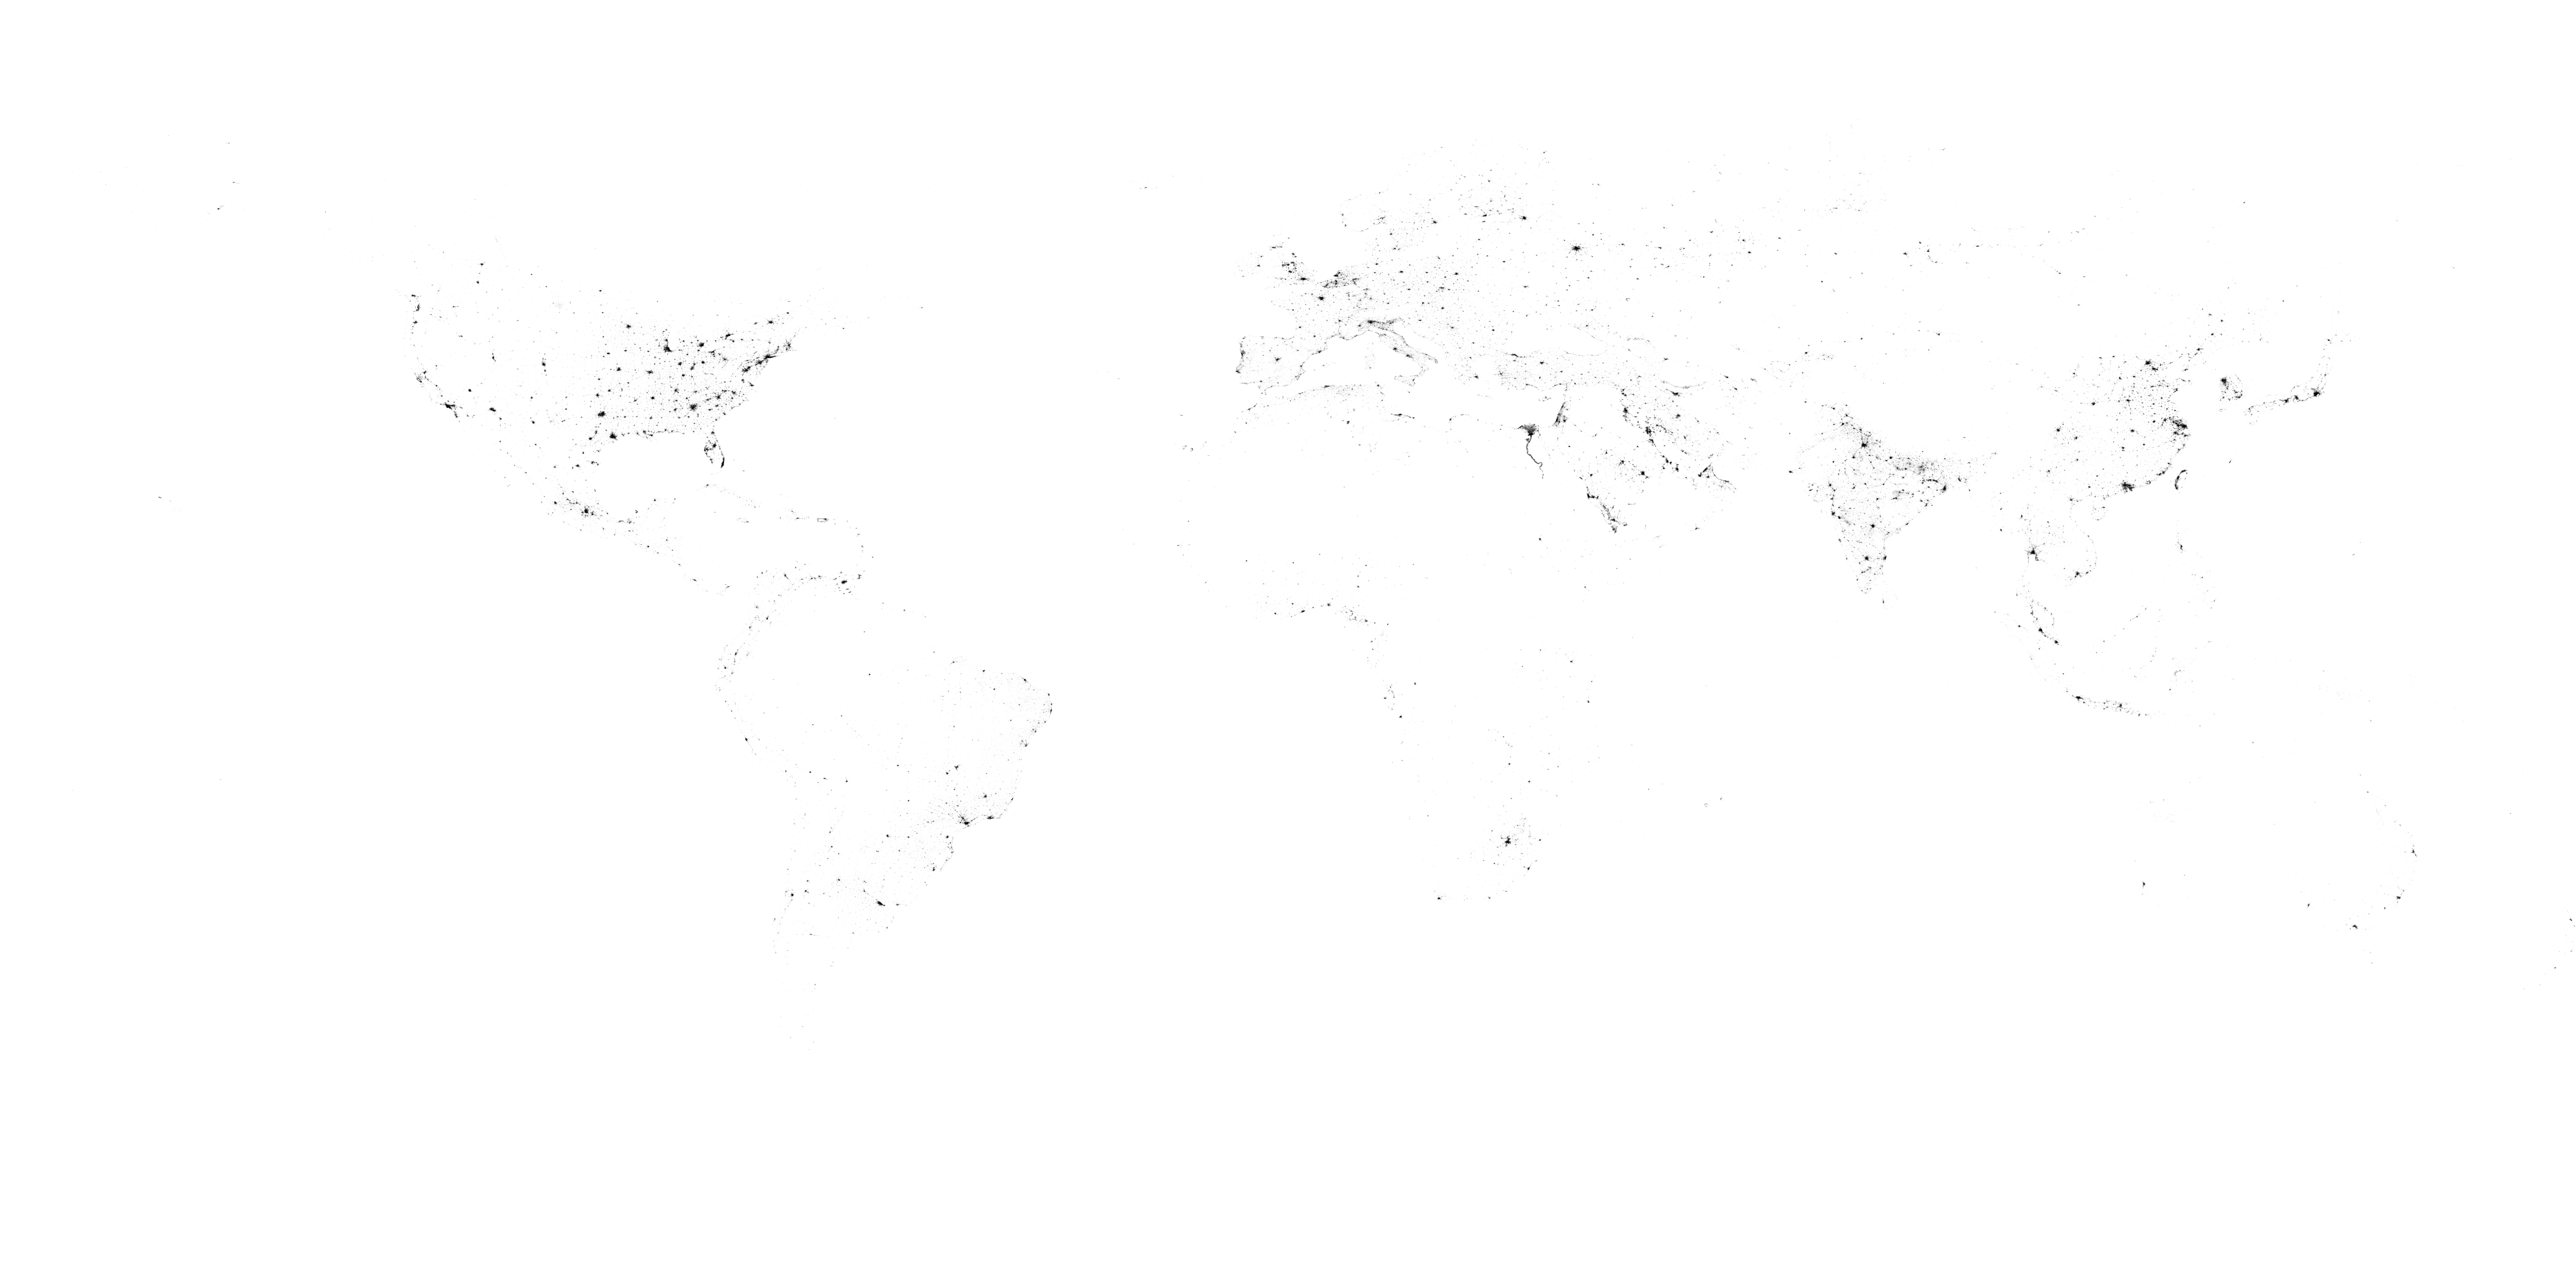
\includegraphics[width=0.8\paperheight, angle=-90, origin=c]{img/tiles_2016_zoom6.png}
	\caption{Image globale annuelle (2016) reconstituée à partir de tuiles téléchargées, puis mise en couleurs négatives.}
	\label{nasa-worldview-tiles}
\end{figure}

Le script Python utilisé se trouve dans Code/scraper/generate\_all.py et nécessite l'installation de la librarie Pillow pour le traitement des images, ainsi qu'urllib pour le téléchargement en soi. Son exécution peut demander plus d'une heure pour le téléchargement (vitesse limitée par le serveur), et plus de 4 Go de RAM pour l'assemblage des tuiles.

\subsubsection{Agence américaine d'observation océanique et atmosphérique}
La source d'images satellite retenue pour la suite du travail est celle de l'Agence américaine d'observation océanique et atmosphérique (abrégé NOAA)\cite{noaa}. Des images satellite nocturnes composites ("Average Lights X Pct") sont disponibles pour les années 1992 à 2013, une période suffisante pour observer des changements depuis l'espace. De plus, ces données sont disponibles en format GeoTIFF, qui contient les informations géographiques nécessaires pour superposer cette carte à sur autre. Il est donc possible d'explorer et manipuler ces cartes à l'aide de logiciels libres tels que QGIS. Il s'agit en réalité des mêmes clichés fournis par Worldview (et Google Earth), mais plus nombreux et dans un format plus exploitable.

Ces images ont été créées en moyennant la valeur de luminosité de chaque pixel sur une année, en ignorant les pixels couverts par des nuages, et en multipliant cette moyenne par la fréquence de détection de lumière sur le pixel au cours de l'année.

\subsection{Grilles de population}
Sedac \cite{sedac} met à disposition des grilles de populations pour le monde entier, sous forme de fichier GeoTIFF. Chaque "case" de 1 km$^2$ est représentée comme un pixel et contient une estimation du nombre de personnes vivant dans cette case. QGIS s'est à nouveau montré d'une grande aide pour visualiser et manipuler ces données volumineuses (exemple en figure \ref{qgis-sedac}).

On remarque que la valeur de densité de population ne varie pas à l'intérieur d'un sous-région. Tous les pixels d'une grande ville ou d'un département possèdent la même valeur. Ces données ont été créées à partir de plusieurs mesures lorsque le décompte de la population pour une sous-région n'a pas été considéré comme fiable. Les images satellites font d'ailleurs partie de ces mesures supplémentaires.

Ces cartes sont disponibles pour les années 2000, 2005, 2010, 2015 et 2020.

\begin{figure}[h]
	\centering
	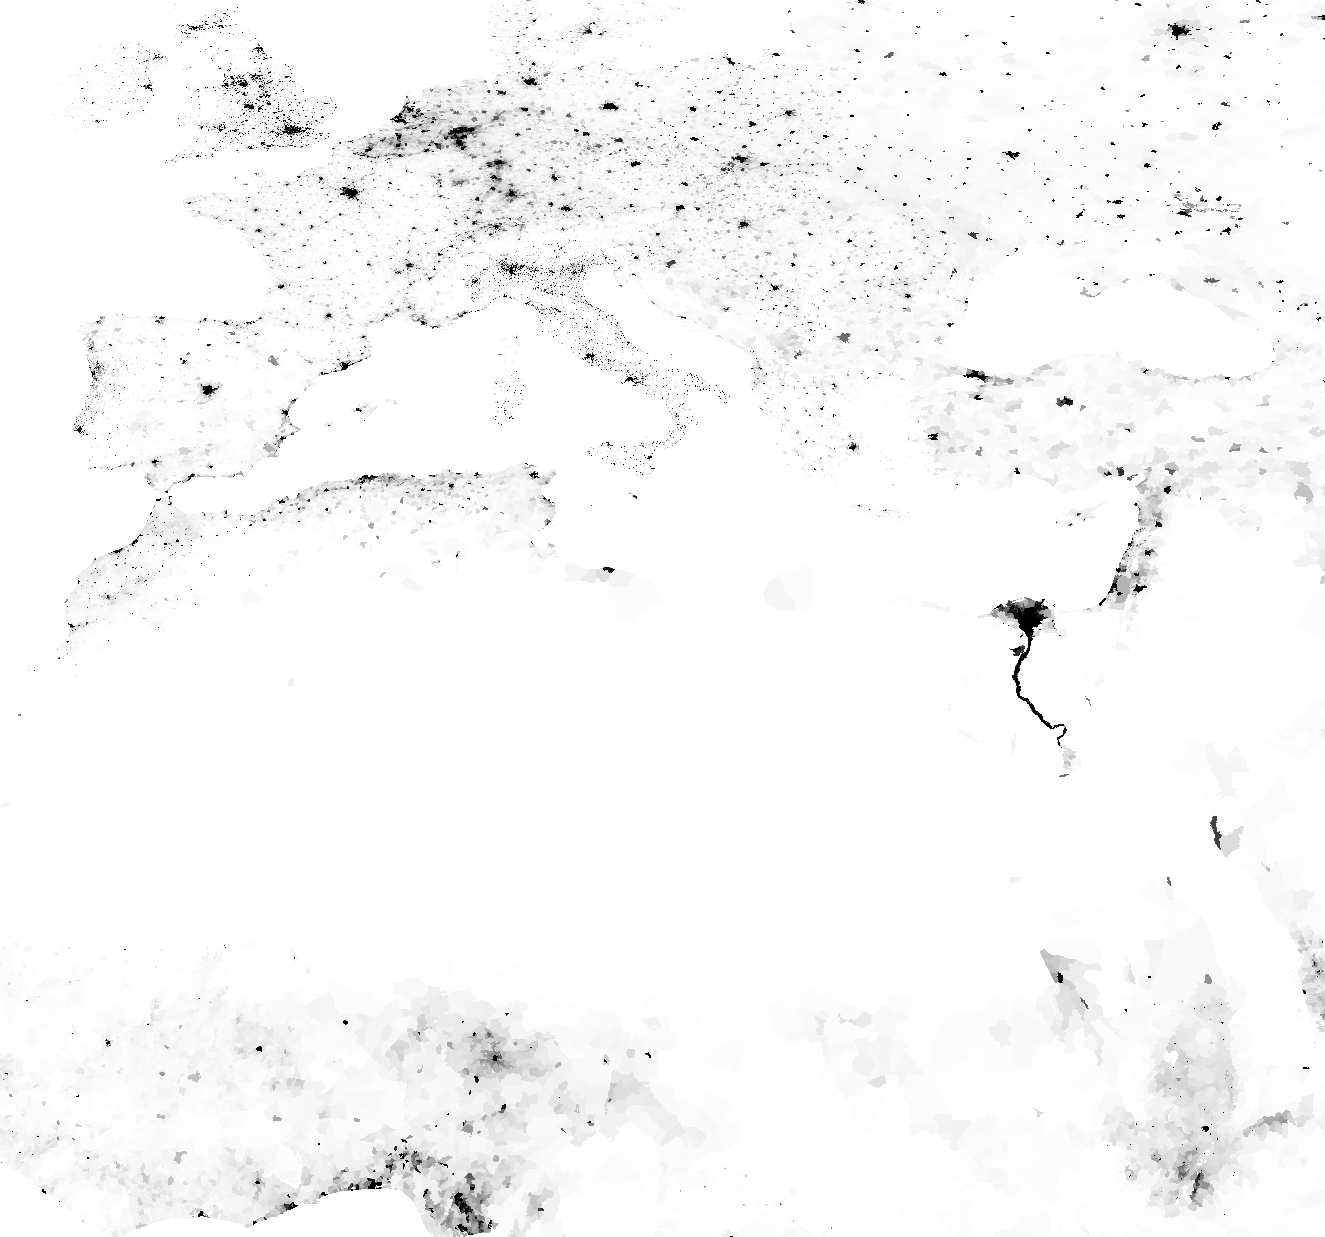
\includegraphics[width=0.8\textwidth]{img/pop_subset.png}
	\caption{Extrait de la grille de population \cite{sedac} rendu avec QGIS. Le blanc indique une absence d'habitants, le noir indique au moins 1000 habitants par kilomètre carré.}
	\label{qgis-sedac}
\end{figure}


\subsection{Pays}
Les grilles de données globales sont difficiles à créer, il n'en existe donc pas pour tous les types et toutes les dates. Afin de contourner ce problème, il y a des outils pour combiner des grilles (ici : l'image satellite) avec des données vectorielles telles que les frontières des pays. L'outil utilisé ici est a librairie Python \texttt{rasterstats}.

Le jeu de données "Admin 0 - Countries" de Natural Earth \cite{naturalearthdata} contient les frontières des pays actuelles, ainsi que des méta-données sur chacun de ces pays (population estimée, indice de développement, différentes appellations et abréviations, etc.). En cas de conflits ou ambiguïté politique sur les frontières, c'est le pays qui contrôle le terrain qui est marqué comme souverain. Voici à quoi ressemblent les méta-données pour la Tunisie :\\
\begin{minipage}[t]{1.0\textwidth}
			{('scalerank', 0), ('featurecla', 'Admin-0 country'), ('LABELRANK', 3.0), ('SOVEREIGNT', 'Tunisia'), ('SOV\_A3', 'TUN'), ('ADM0\_DIF', 0.0), ('LEVEL', 2.0), ('TYPE', 'Sovereign country'), ('ADMIN', 'Tunisia'), ('ADM0\_A3', 'TUN'), ('GEOU\_DIF', 0.0), ('GEOUNIT', 'Tunisia'), ('GU\_A3', 'TUN'), ('SU\_DIF', 0.0), ('SUBUNIT', 'Tunisia'), ('SU\_A3', 'TUN'), ('BRK\_DIFF', 0.0), ('NAME', 'Tunisia'), ('NAME\_LONG', 'Tunisia'), ('BRK\_A3', 'TUN'), ('BRK\_NAME', 'Tunisia'), ('BRK\_GROUP', None), ('ABBREV', 'Tun.'), ('POSTAL', 'TN'), ('FORMAL\_EN', 'Republic of Tunisia'), ('FORMAL\_FR', None), ('NAME\_CIAWF', 'Tunisia'), ('NOTE\_ADM0', None), ('NOTE\_BRK', None), ('NAME\_SORT', 'Tunisia'), ('NAME\_ALT', None), ('MAPCOLOR7', 4.0), ('MAPCOLOR8', 3.0), ('MAPCOLOR9', 3.0), ('MAPCOLOR13', 2.0), ('POP\_EST', 11403800.0), ('POP\_RANK', 14.0), ('GDP\_MD\_EST', 130800.0), ('POP\_YEAR', 2017.0), ('LASTCENSUS', 2004.0), ('GDP\_YEAR', 2016.0), ('ECONOMY', '6. Developing region'), ('INCOME\_GRP', '3. Upper middle income'), ('WIKIPEDIA', -99.0), ('FIPS\_10\_', 'TS'), ('ISO\_A2', 'TN'), ('ISO\_A3', 'TUN'), ('ISO\_A3\_EH', 'TUN'), ('ISO\_N3', '788'), ('UN\_A3', '788'), ('WB\_A2', 'TN'), ('WB\_A3', 'TUN'), ('WOE\_ID', 23424967.0), ('WOE\_ID\_EH', 23424967.0), ('WOE\_NOTE', 'Exact WOE match as country'), ('ADM0\_A3\_IS', 'TUN'), ('ADM0\_A3\_US', 'TUN'), ('ADM0\_A3\_UN', -99.0), ('ADM0\_A3\_WB', -99.0),	 ('CONTINENT', 'Africa'), ('REGION\_UN', 'Africa'), ('SUBREGION', 'Northern Africa'), ('REGION\_WB', 'Middle East \& North Africa'), ('NAME\_LEN', 7.0), ('LONG\_LEN', 7.0), ('ABBREV\_LEN', 4.0), ('TINY', -99.0), ('HOMEPART', 1.0), ('MIN\_ZOOM', 0.0), ('MIN\_LABEL', 3.0), ('MAX\_LABEL', 8.0)}
\end{minipage}\\

Le script Code/regionovertime/dumpstats.py superpose ces données vectorielles à l'image satellite pour ajouter à chaque pays sa luminosité moyenne sur une échelle de 0 à 63 ainsi que l'écart-type de luminosité par pixel. Puis ces données sont enregistrées dans le fichier stats.pickle pour être utilisées plus tard.

Grâce à cette information sur la luminosité perçue par pays, on peut faire un parallèle avec une grande variété de données, telles que le produit intérieur brut (GDP), la consommation en énergie, le niveau de développement, l'indice économique, les émissions de C0$_2$, etc.

La source utilisée pour les données de population par pays et par année vient du site du Département des Affaires Économiques et Sociales des Nations Unies \cite{un-wpp}, plus précisément de la feuille Excel "Total Population - Both Sexes" de 2017.

La source de données pour le produit intérieur brut en USD par année est fournie par The World Bank \cite{theworldbank} et téléchargée depuis \url{http://data.un.org/Data.aspx?q=gdp&d=WDI&f=Indicator_Code%3aNY.GDP.MKTP.CD} (visité le 07.06.2018, dernière mise à jour le 12.10.2016).

Les données sur la consommation en électricité en millions de kWh par pays et par année sont tirées de \url{http://data.un.org/Data.aspx?d=EDATA&f=cmID%3AEL} (données issues de la Division Statistique des Nations Unies, mises à jour en janvier 2018). Le filtre "Electricity - Final energy consumption" a été utilisé pour ne garder que la consommation totale, sans les nombreux détails proposés par la base de données sur l'usage de l'électricité.

\section{Recherche de corrélation}
\subsection{Pays}
La superposition de deux grilles (population et image satellite) de dimensions différentes n'est pas évidente, c'est pourquoi les première données à avoir été mises en parallèles dans ce travail sont la population par pays \cite{un-wpp}, le produit intérieur brut \cite{theworldbank}, et la luminosité totale du pays perçue depuis l'espace (extraite par script Python à partir des vecteurs de frontières de Natural Earth \cite{naturalearthdata} et des images de la NOAA \cite{noaa}).

Pour chaque année disponible (1992-2013), il est donc possible de dessiner pour la majorité des pays les histogrammes de luminosité, population et PIB (examples en figures \ref{sum_France}, \ref{sum_China}, \ref{sum_Japan} et \ref{sum_Armenia}). Cette représentation n'est pas idéale car l'échelle n'est pas constante entre les pays. Ce qui apparait comme une grande variation de luminosité peut ne pas en être du tout. Certains pays ne portent pas exactement le même nom dans tous les jeux de données, ils sont donc mis de côté dans les résultats.

La figure \ref{sum_France} est typique des résultats obtenus. Elle laisse présager une forte corrélation entre les trois données observées. Cependant, la figure \ref{sum_China} soulève déjà des doutes : la population croît de façon linéaire, mais le PIB et la lumière perçue augmentent de plus en plus vite. Les graphes du Japon (figure \ref{sum_Japan}) semblent indiquer que la luminosité suit le PIB également lorsque ce dernier diminue. Enfin le cas de l'Arménie (figure \ref{sum_Armenia}) nous pousse à croire que le PIB a une corrélation plus forte que la population avec la luminosité.

Jusqu'ici, rien n'est confirmé. Nous ne possédons que des observations par pays sur des échelles variables qui sont regroupées par pays, ce qui représente une résolution plutôt basse. Sans parler de fait que 320 pays sur 21 années n'est pas une quantité de données acceptable pour entraîner un réseau de neurones.

\begin{figure}
	\centering
	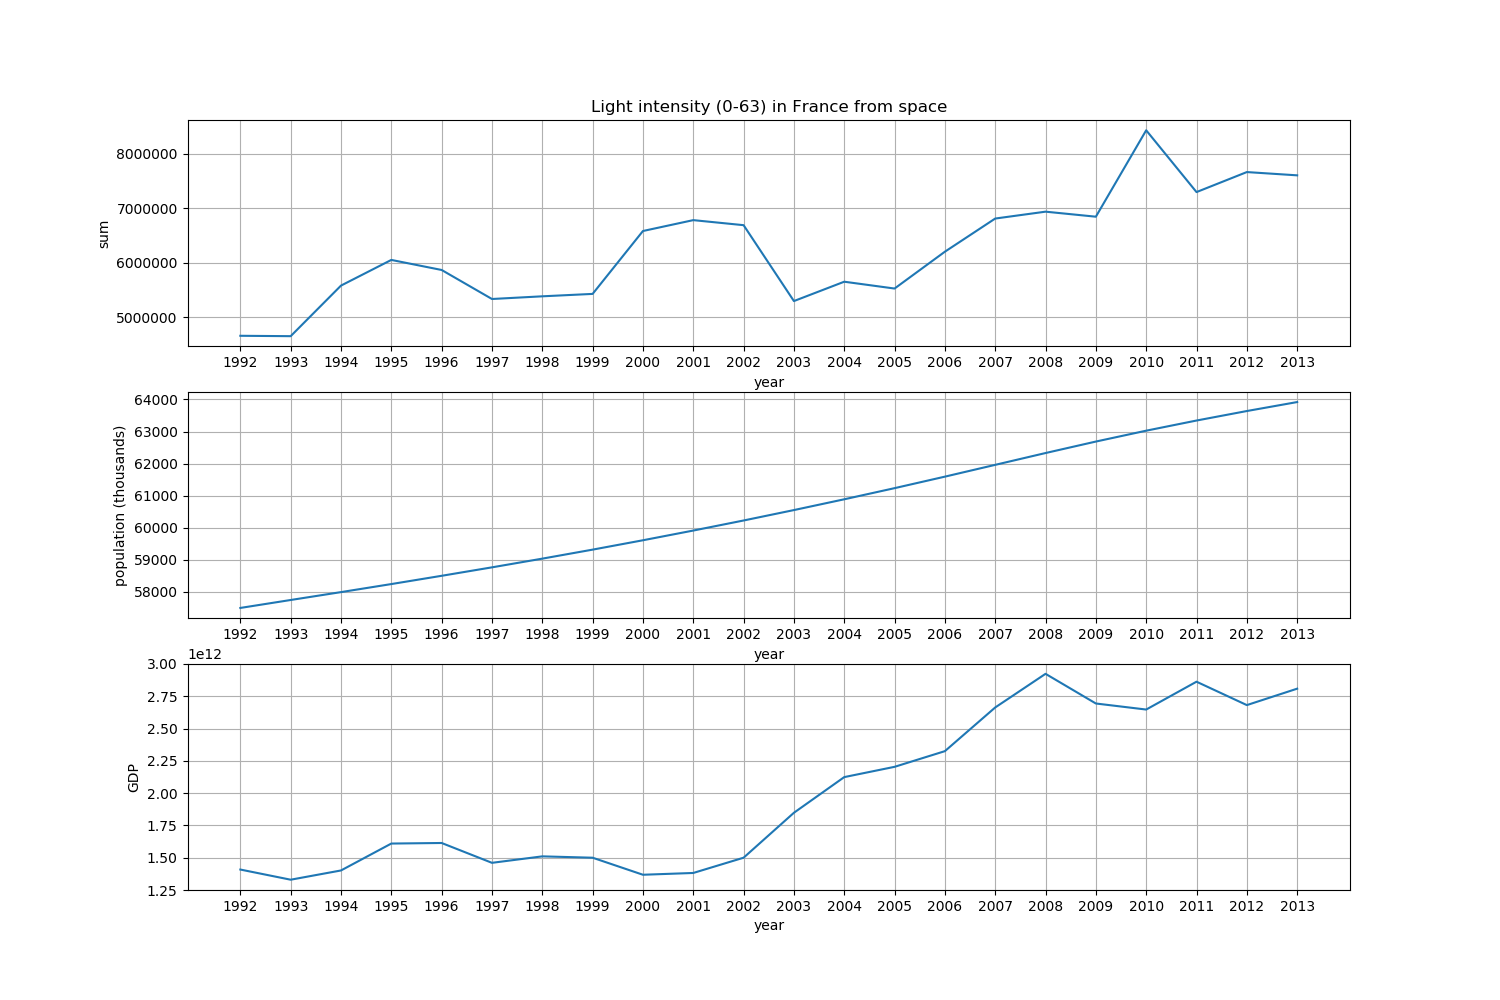
\includegraphics[width=1.0\textwidth]{img/sum_France.png}
	\caption{Quantité de lumière perçue depuis l'espace, population et PIB de la France entre 1992 et 2013.}
	\label{sum_France}
\end{figure}

\begin{figure}
	\centering
	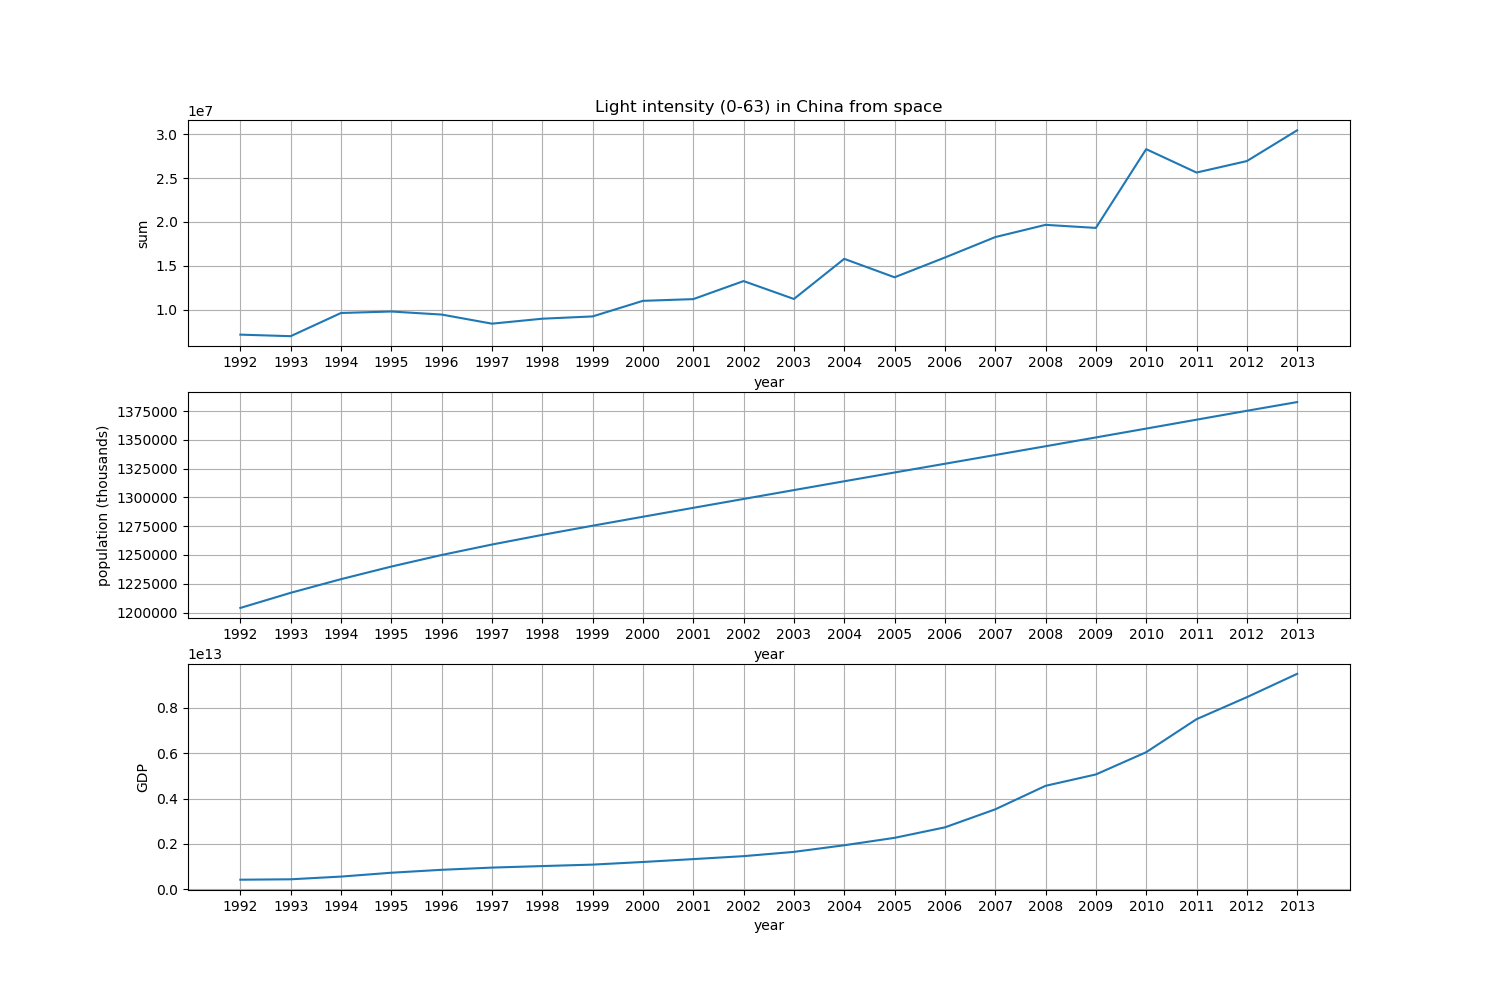
\includegraphics[width=1.0\textwidth]{img/sum_China.png}
	\caption{Quantité de lumière perçue depuis l'espace, population et PIB de la Chine entre 1992 et 2013.}
	\label{sum_China}
\end{figure}


\begin{figure}
	\centering
	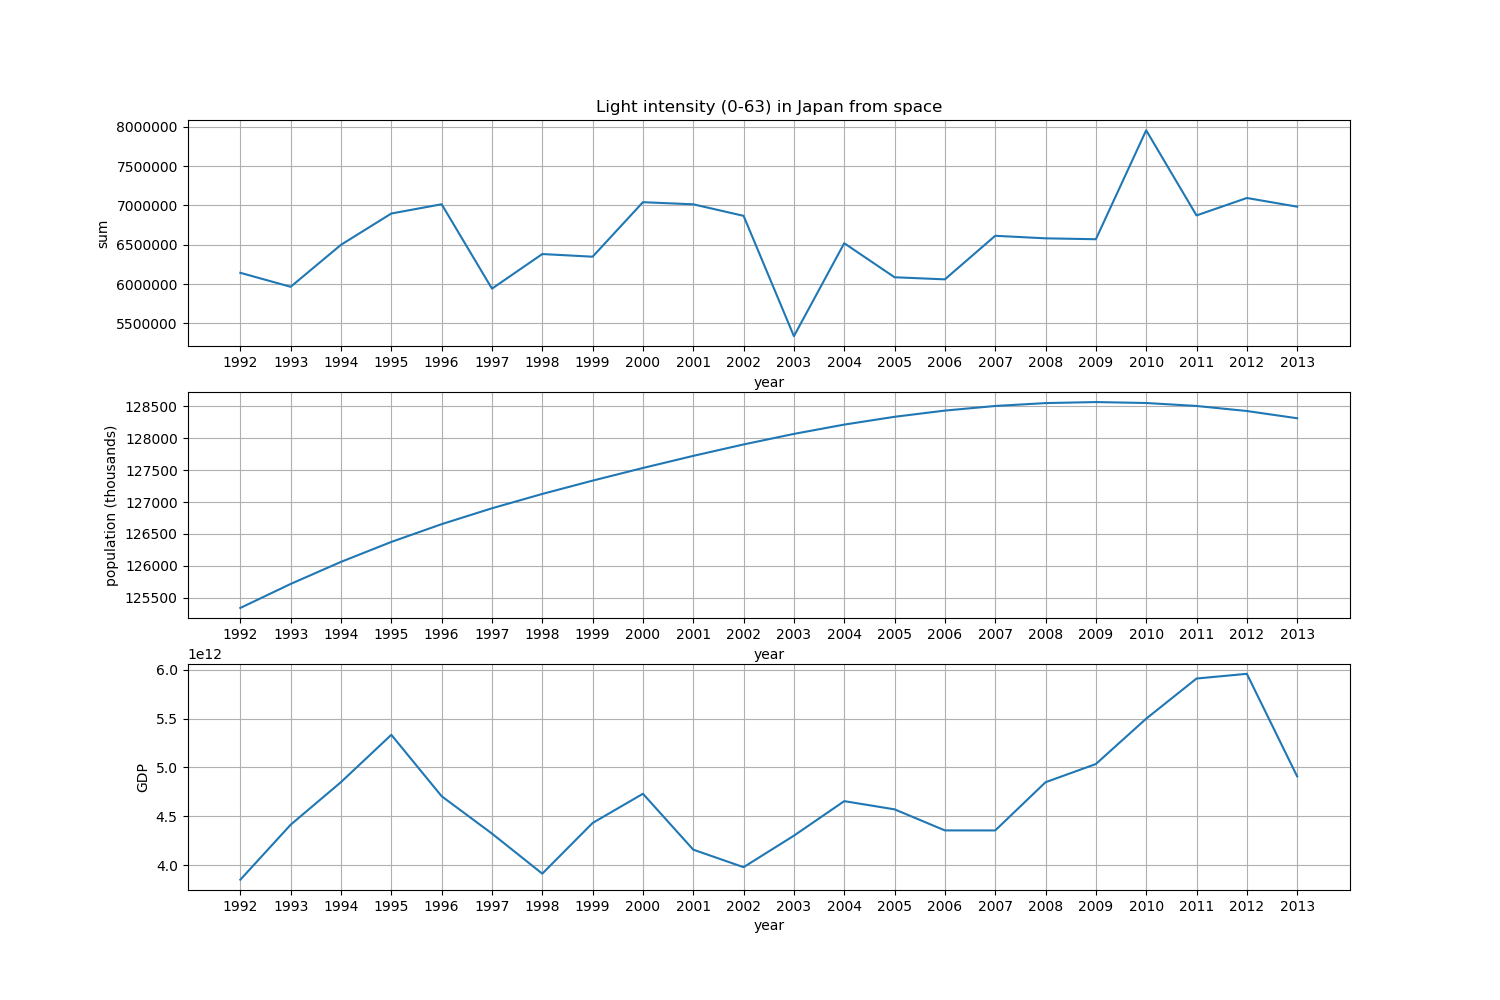
\includegraphics[width=1.0\textwidth]{img/sum_Japan.png}
	\caption{Quantité de lumière perçue depuis l'espace, population et PIB du Japon entre 1992 et 2013.}
	\label{sum_Japan}
\end{figure}


\begin{figure}
	\centering
	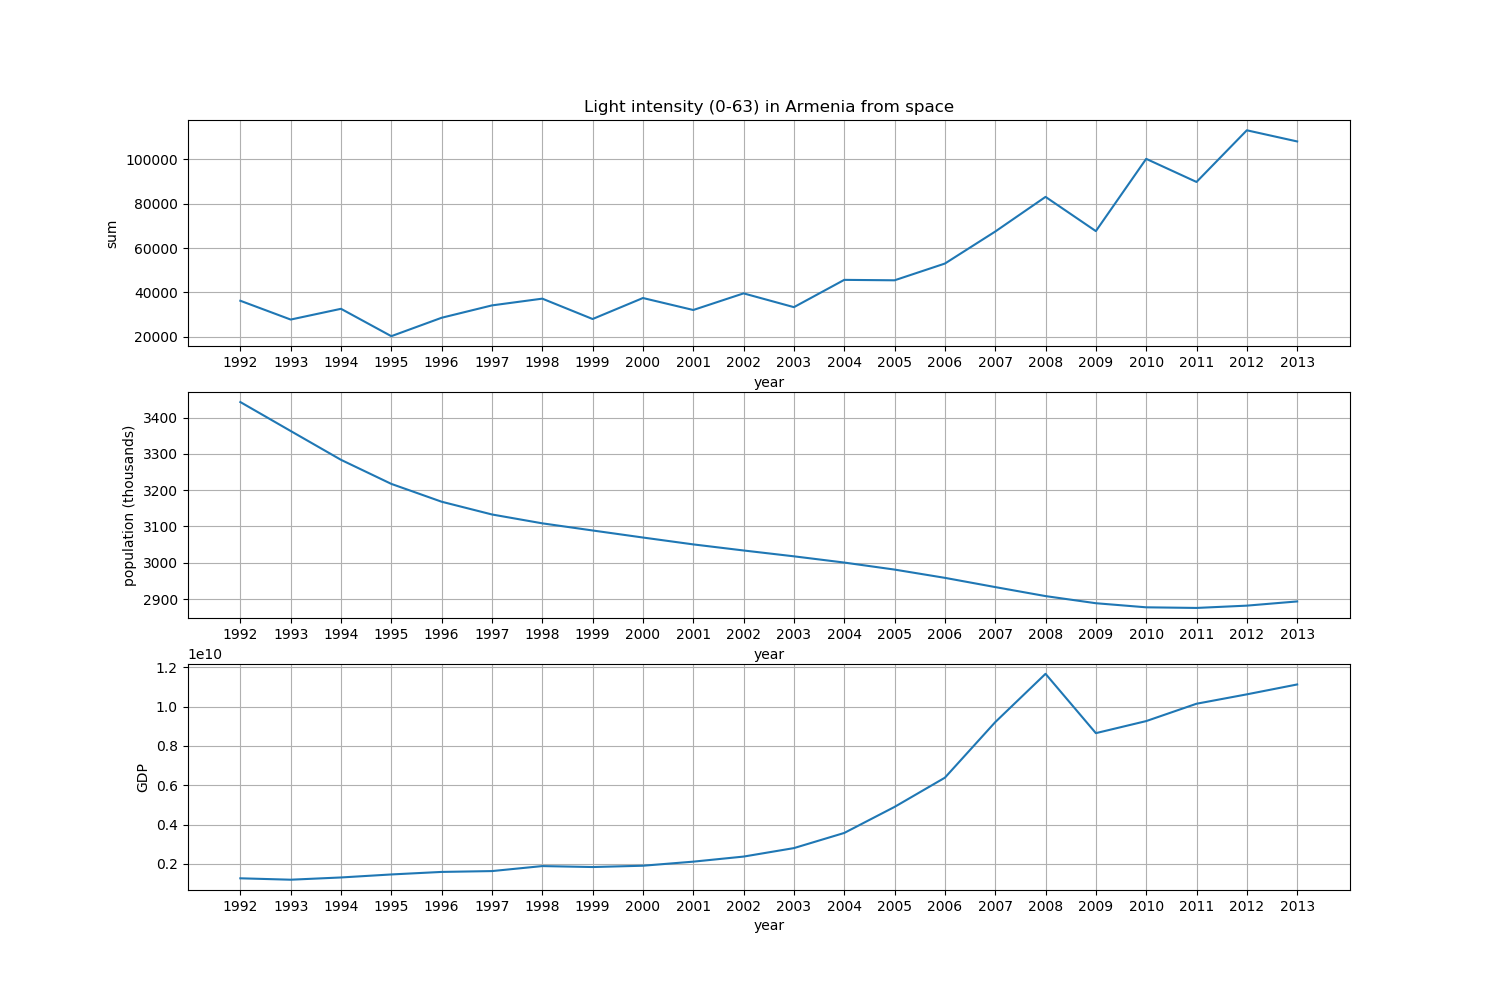
\includegraphics[width=1.0\textwidth]{img/sum_Armenia.png}
	\caption{Quantité de lumière perçue depuis l'espace, population et PIB de l'Arménie entre 1992 et 2013.}
	\label{sum_Armenia}
\end{figure}

Il est également possible de générer des nuages de points comparant la lumière émise et, au choix, l'énergie consommée, la population du pays ou le PIB, et de colorer ces points par indice de développement économique (tiré des données vectorielles Natural Earth \cite{naturalearthdata}).

Le premier de ces nuages de points compare la luminosité et la population de 2013 pour chaque pays (figure \ref{country_lightpop_scatter}). On observe immédiatement qu'il existe une corrélation. Son coefficient de Pearson est 0.56. On ne peut pas encore déterminer s'il y a une relation directe, ou si ces deux variables sont simplement corrélées à la taille du territoire. En effet, on ne fait que sommer la population et la quantité de lumière émise, on ne calcule pas de moyenne par pays.
Sans surprise, on voit également que les pays ayant un index économique élevé émettent plus de lumière que d'autres pays à population équivalente.

\begin{figure}
	\centering
	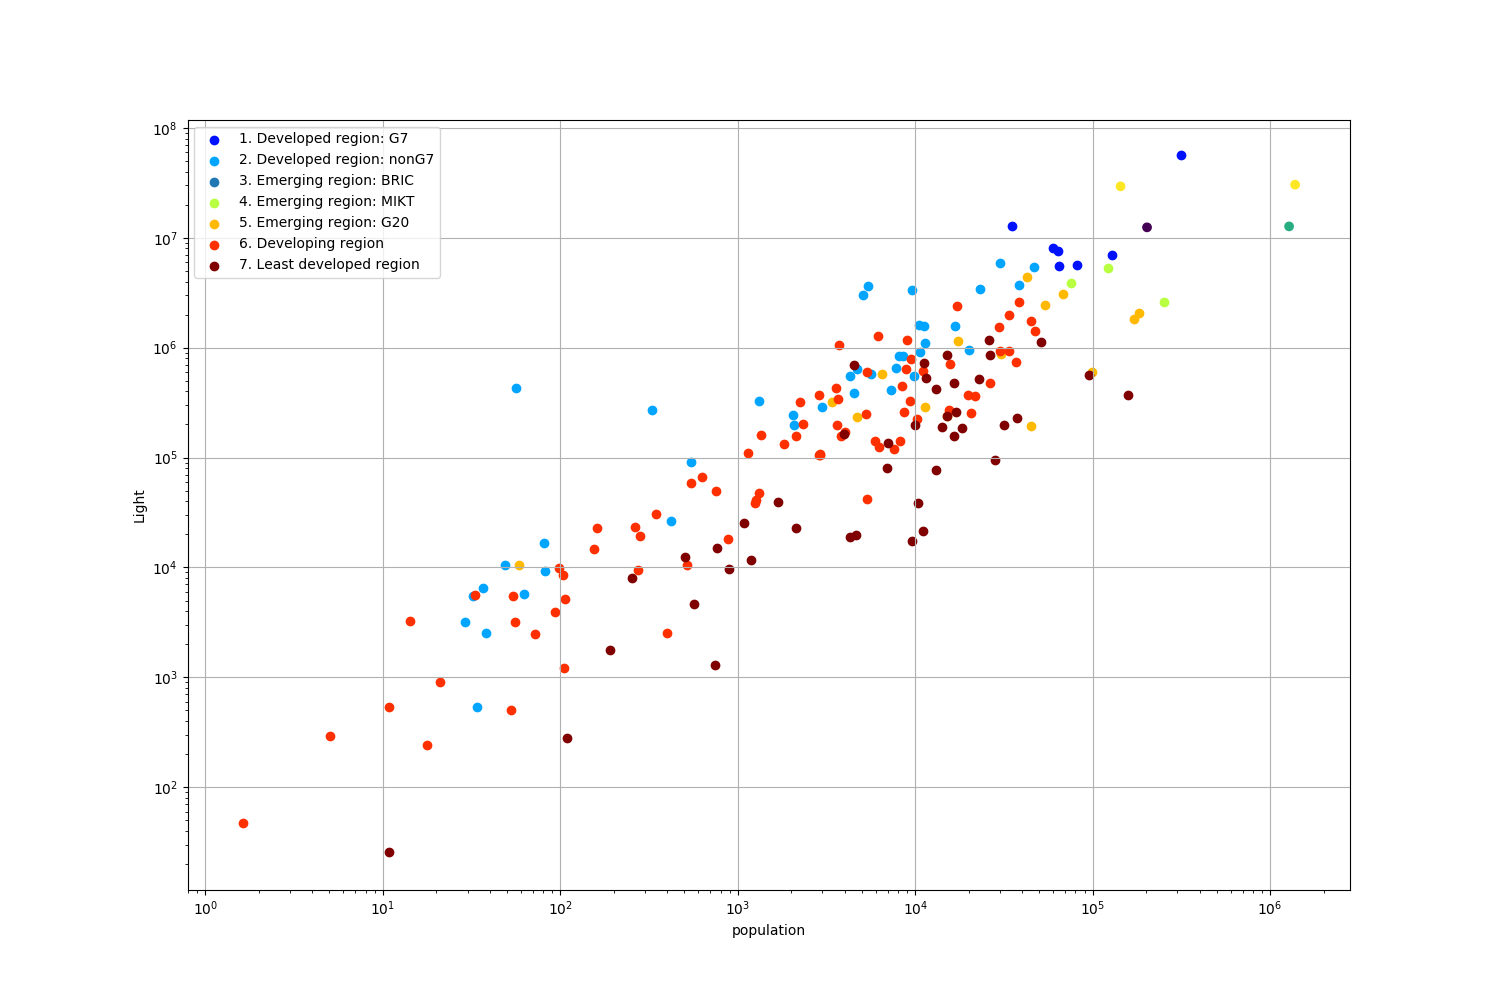
\includegraphics[width=1.0\textwidth]{img/population-light.png}
	\caption{Pays placés par population et luminosité totale émise sur une échelle logarithmique, colorés par indice économique.}
	\label{country_lightpop_scatter}
\end{figure}

Le deuxième graphe généré est beaucoup plus intéressant car il compare le produit intérieur brut de chaque pays avec leur émission de lumière (figure \ref{country_gdppop_scatter}). On observe une forte corrélation, dont le coefficient de Pearson est 0.819.
Naturellement, l'indice de développement économique est très corrélé avec le PIB (\textit{GDP} en Anglais).

\begin{figure}
	\centering
	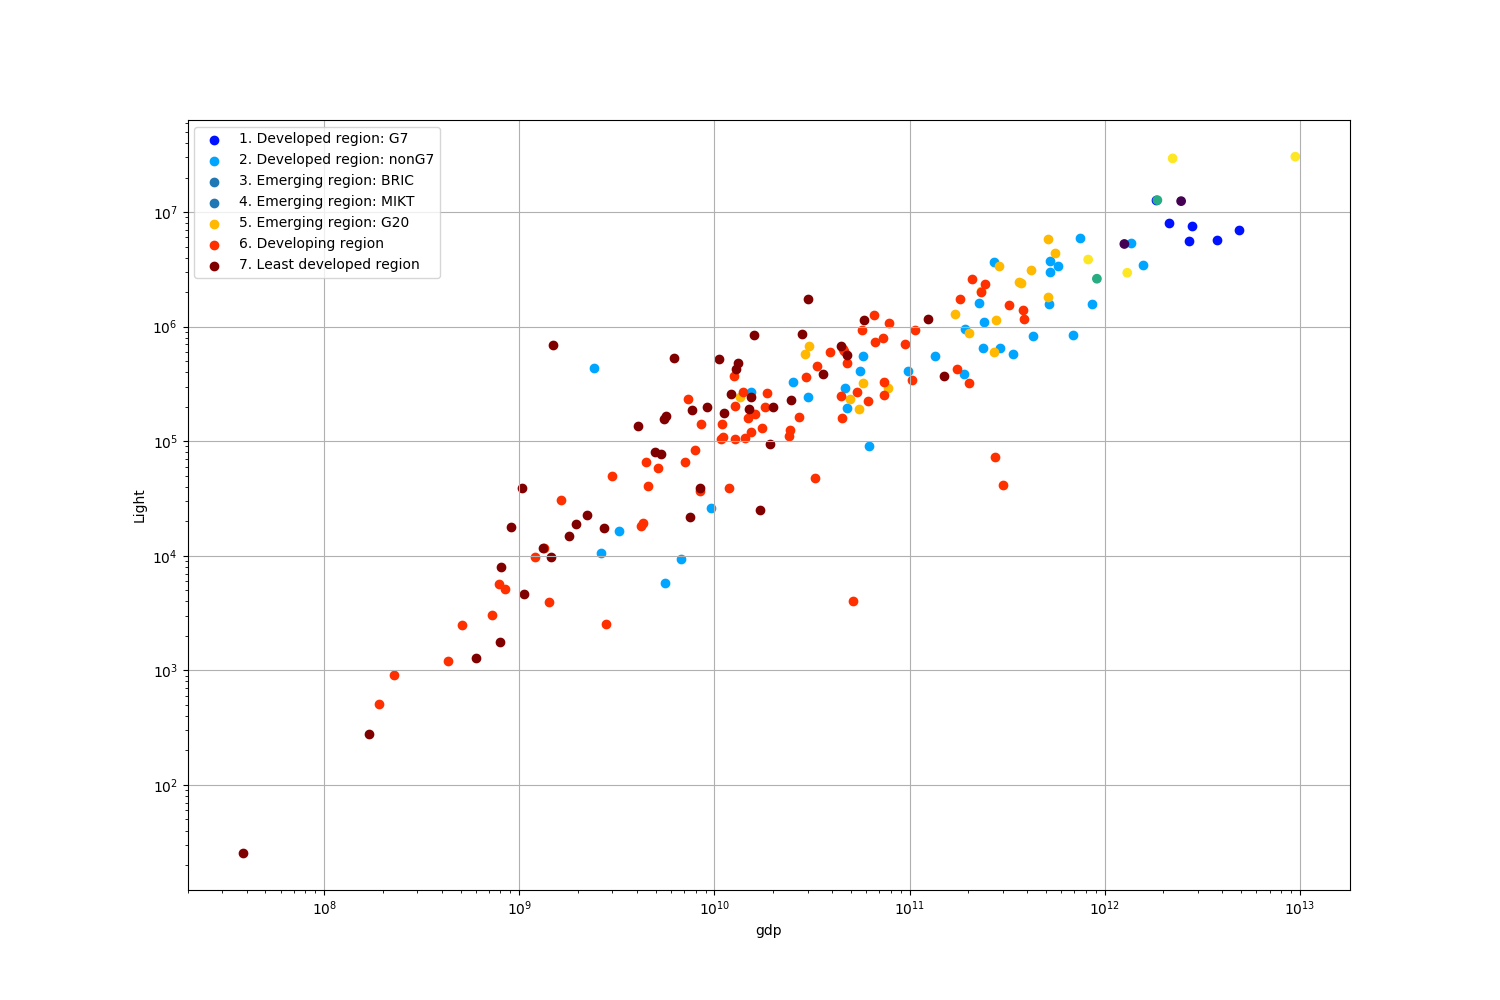
\includegraphics[width=1.0\textwidth]{img/gdp-light.png}
	\caption{Pays placés par PIB en USD et luminosité totale émise sur une échelle logarithmique, colorés par indice économique.}
	\label{country_gdppop_scatter}
\end{figure}

Une autre comparaison est possible avec la consommation en électricité, illustrée en figure \ref{country_energypop_scatter}. La forte corrélation (coefficient de 0.81) entre émission de lumière et consommation d'énergie n'est pas une surprise, mais on remarque un phénomène intéressant avec l'index économique des pays. Les pays en voie de développement ont tendance à émettre beaucoup plus de lumière pour une consommation d'électricité équivalente aux pays développés. On peut spéculer sur les causes d'une telle différence (data centers, chauffages, etc.) mais ce n'est pas l'objet de ce travail.

\begin{figure}
	\centering
	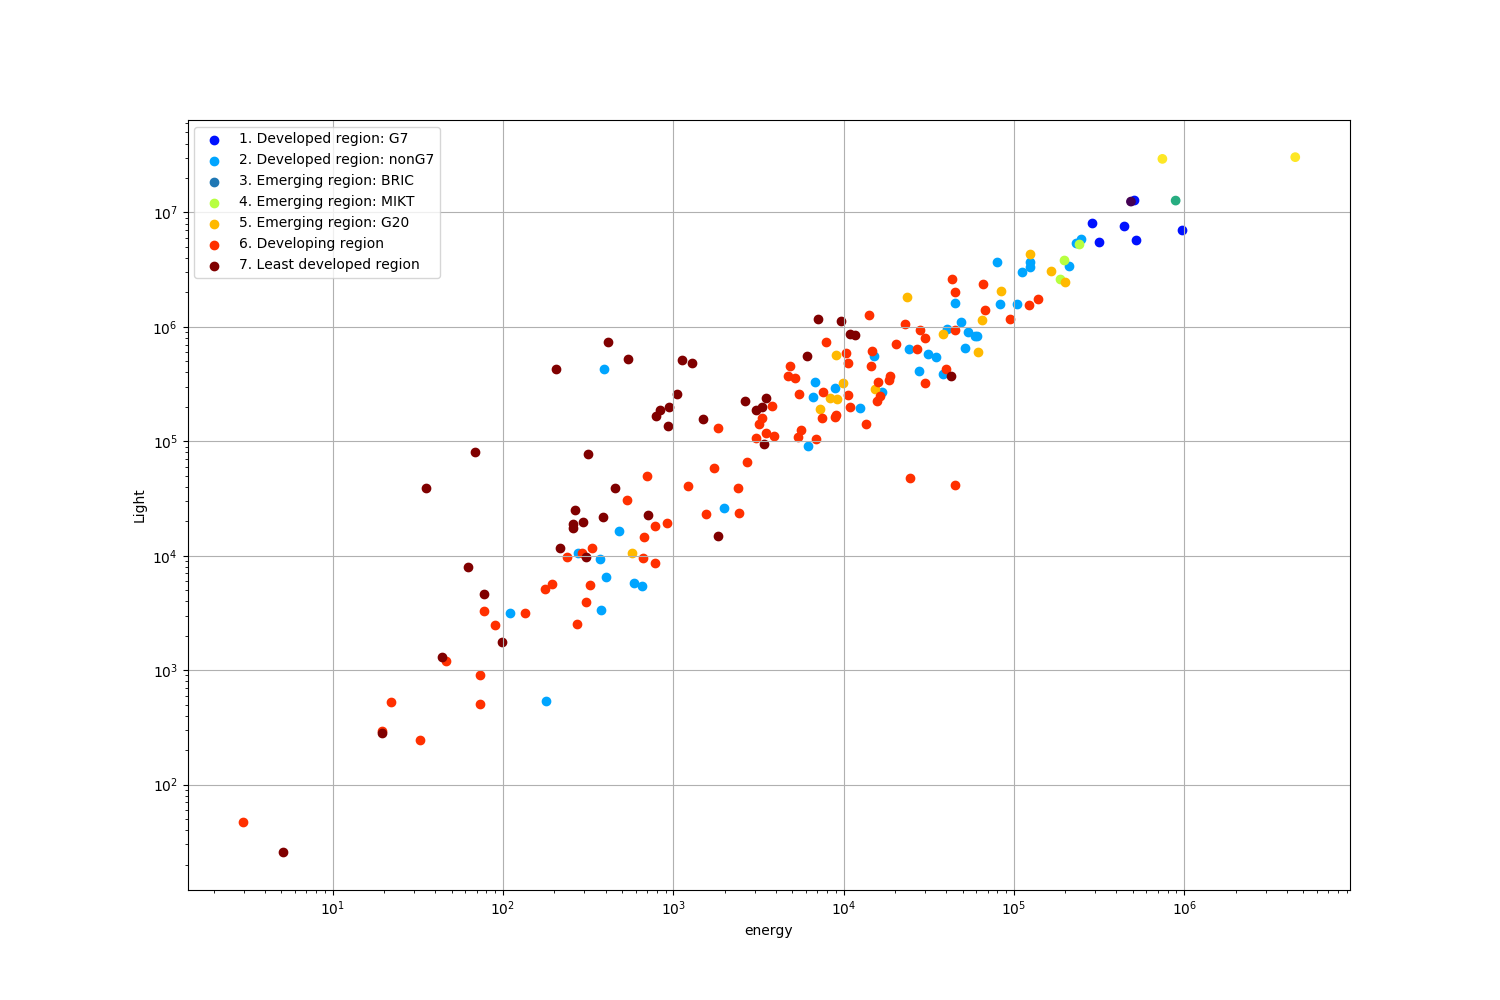
\includegraphics[width=1.0\textwidth]{img/energy-light.png}
	\caption{Pays placés par consommation en électricité en millions de kWh et luminosité totale émise sur une échelle logarithmique, colorés par indice économique.}
	\label{country_energypop_scatter}
\end{figure}

\subsection{Grille de population}

Après avoir tenté de programmer un script Python pour superposer deux grilles de dimensions différentes, il s'est avéré que l'application QGIS est capable d'effectuer cette opération. Il suffit de :

\begin{itemize}
	\item Ouvrir les grilles avec QGIS : population et image satellite. Elles doivent apparaitre dans la liste des couches.
	\item Dans la barre d'outils, choisir "Raster" $\rightarrow$ Divers $\rightarrow$ Fusionner.
	\item Cocher l'option "Placer chaque fichier en entrée dans une bande séparée." puis lancer la fusion "Run in Background".
\end{itemize}

La grille résultante contient donc environ 800 millions de pixels (possédant chacun une valeur de population et de luminosité) qui sont potentiellement autant de données d'entraînement pour chaque année disponible (2000, 2005, 2010, qui correspondent aux dates des grilles de population). Après avoir ajusté ses propriétés d'affichage et inversé les couleurs, on obtient la figure \ref{lightpop_2000}. Le bleu ciel correspond à la lumière visible depuis l'espace, le rose la population (sur une échelle de 1 à 1000 habitants par km$^2$). Le bleu foncé correspond au chevauchement des deux couleurs. On peut déjà observer que, si la luminosité ne suit pas l'évolution de la population dans le temps à l'échelle d'un pays, elle est tout de même concentrée géographiquement sur les points les plus peuplés.

\begin{figure}
	\centering
	\includegraphics[width=0.8\paperheight, angle=-90, origin=c]{img/lightpop_2000.png}
	\caption{Superposition de l'image satellite nocturne (bleu ciel) et de la grille de population (rose).}
	\label{lightpop_2000}
\end{figure}

Si on pose chaque pixel sur un nuage de point dont les axes sont la luminosité et la population, on obtient la figure \ref{lightpop_scatter}. On constate qu'il sera très difficile de deviner la valeur de population à partir de l'intensité lumineuse d'un seul pixel. Cela nous oriente donc plutôt dans la direction d'un réseau de neurones à convolutions, qui considère les pixels par groupes.

\begin{figure}
	\centering
	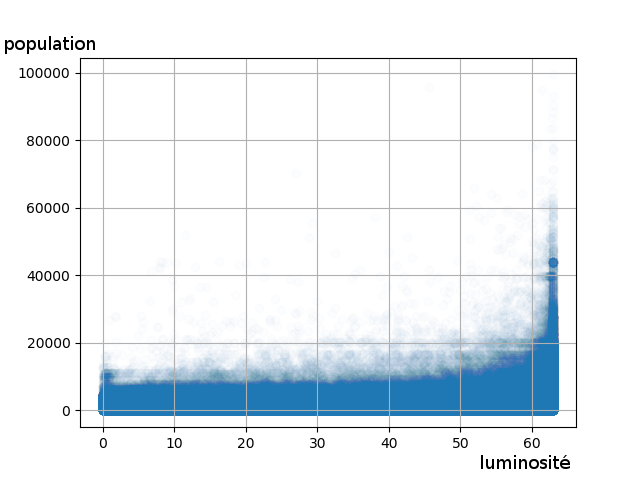
\includegraphics[width=0.7\textwidth]{img/lightpop_scatter.png}
	\caption{Valeur de luminosité et de population pour chaque km$^2$ (année 2000)}
	\label{lightpop_scatter}
\end{figure}

\section{Données à explorer}
Parmi les données potentiellement intéressantes qui n'ont pas encore été explorées dans ce travail, il y a notamment des grilles pour :
\begin{itemize}
	\item l'impact humain sur l'environnement,
	\item l'estimation des populations haute résolution de Facebook (digital globe),
	\item les changements de luminosité d'une année à l'autre (à calculer à partir des images satellites),
	\item la couverture du territoire (vert ou bétonné),
\end{itemize}
Toutes les sources de données satellite n'ont par ailleurs pas été explorées. NOAA dispose d'autres images composites, plus récentes et exposant d'autres fréquences du spectre lumineux.

\chapter{Modèle}
\section{Environnement de développement}
Python est un langage largement utilisé pour manipuler des données et faire de l'apprentissage automatique. Il dispose de librairies optimisées précisément pour cette tâche, dont Keras.

Keras est une librairie Python open source permettant le prototypage rapide de réseaux de neurones et peut fonctionner au-dessus de TensorFlow (open source et développé par Google), CNTK ou Theano. Une fonctionnalité très attractive de TensorFlow est l'exploitation automatique du processeur graphique s'il est disponible. En effet, ces processeurs sont très performants pour l'apprentissage automatique, car c'est un travail hautement parallélisable.

Afin d'activer l'utilisation d'un GPU Nvidia par Tensorflow sur Windows 10, il faut installer la librairie tensorflow-gpu, le CUDA Toolkit de Nvidia en version 9.0 et le SDK cuDNN (\textit{CUDA Deep Neural Network library}) de Nvidia en version 7.0 (instructions détaillées : \url{https://www.tensorflow.org/install/install_linux}).

\section{Réseau de neurones}
Pour commencer à développer le réseau de neurones, on commencera par tenter de prédire la population d'une petite région (une tuile) à partir de l'image satellite de l'année 2005, en entraînant la machine sur celle de 2000 et la grille de population correspondante \cite{sedac}.

Comme on a pu observer que la prédiction à partir d'un pixel isolé n'est pas réaliste, on aimerait prendre en compte les valeurs des pixels voisins. En effet, s'il y a beaucoup de pixels proches illuminés, il y a de meilleures chances pour que la région soit densément peuplée que si un seul pixel est illuminé. De plus, si le réseau de neurones peut reconnaître les formes, il sera en mesure de différencier le centre et la périphérie d'une ville, ainsi que des routes ou villages isolés.

Le système qui répond à ces exigences est le réseau de neurones à convolutions. Cependant, alors que l'usage habituel d'un tel réseau sert à la classification de données, on a besoin ici d'obtenir un nombre réel. Il s'agit d'adapter le système pour faire de la régression, ce que l'on fait lorsqu'on compte le nombre de voitures sur un parking par exemple.

Avant de commencer l'entraînement, on découpe l'image satellite nocturne en tuiles de 32 sur 32 pixels (1024 km$^2$). Chacune de ces tuiles sera considéré comme une observation à donner en entrée du modèle. La sortie sera une valeur réelle correspondant au nombre d'habitants dans la zone donnée en entrée.

\section{Méta-paramètres}

\begin{figure}
	\centering
	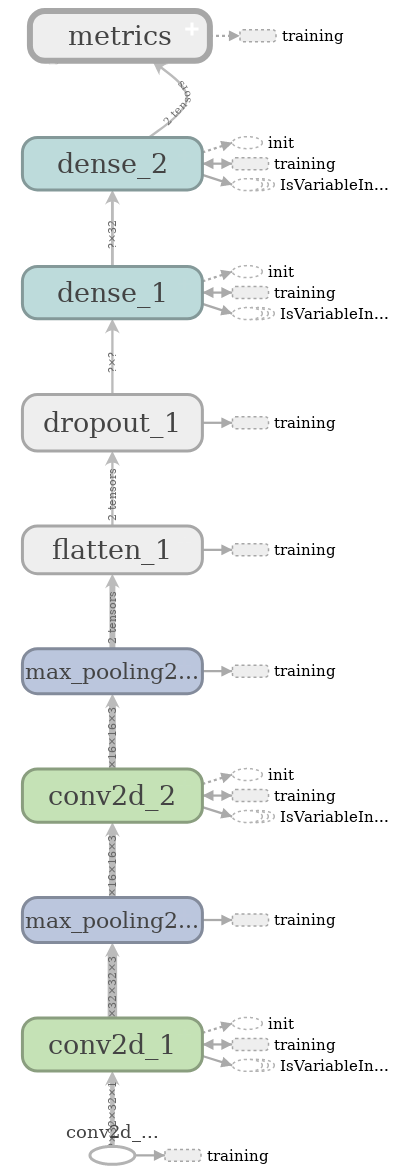
\includegraphics[height=0.7\textheight]{img/net1.png}
	\caption{Topologie de la toute première version du réseau de neurones.}
	\label{net1}
\end{figure}

La topologie du réseau (figure \ref{net1}) s'inspire grossièrement du travail effectué par l'Arnhold Institute for Global Health \cite{netpop-article}, qui consiste à estimer les populations de petites régions à partir d'images satellite de jour \textit{et} de nuit.

Les couches sont définies comme suit :
\begin{itemize}
	\item Convolution de 32 filtres, chaque kernel fait 3x3 pixels, fonction d'activation ReLU,
	\item MaxPooling pour diviser par 2 la largeur et la hauteur de la tuile,
	\item Convolution identique à la première couche,
	\item Flatten,
	\item Dropout de 20\% pour réduire les chances d'overfitting,
	\item Couche dense de 32 neurones,
	\item Couche dense d'un seul neurone, qui correspond à la sortie du modèle.
\end{itemize}

L'optimiseur utilisé est Adam. C'est généralement un bon choix par défaut grâce à sa performance en terme de vitesse de calcul, et à sa capacité à répondre aux besoins d'un grand nombre de problèmes. Le \textit{learning rate} choisi (après quelques essais) est 0.001. Enfin, la fonction objectif à optimiser est la moyenne des erreurs au carré.

\section{Résultats}

Les résultats suivants ont été obtenus en entraînant le modèle sur une région couvrant l'Europe de l'Ouest et l'Afrique du Nord en l'an 2000. La phase de test est effectuée sur l'Amérique du Nord et une partie de l'Amérique du Sud en l'an 2005.

\begin{figure}
	\centering
	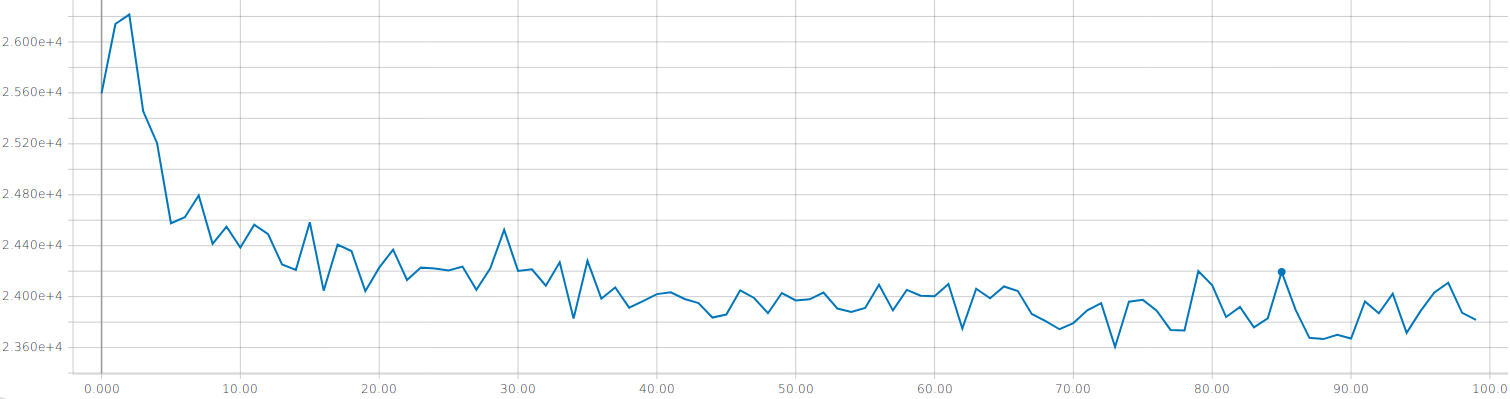
\includegraphics[width=1.0\textwidth]{img/mae1.png}
	\caption{Moyennes des erreurs absolues sur 100 itérations.}
	\label{mae1}
\end{figure}

\begin{figure}
	\centering
	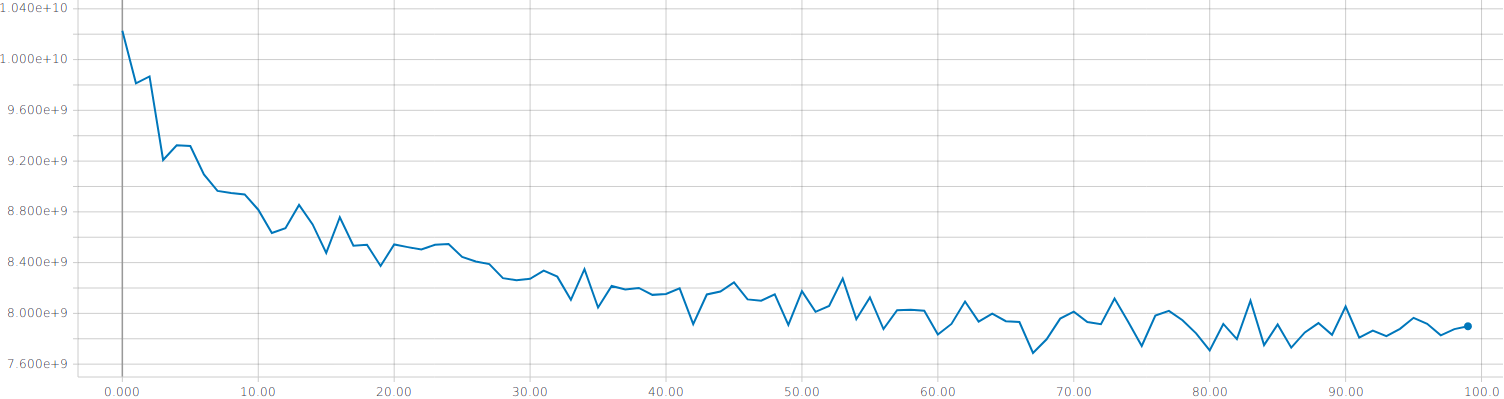
\includegraphics[width=1.0\textwidth]{img/mse1.png}
	\caption{Moyennes des erreurs au carré (fonction objectif) sur 100 itérations.}
	\label{mse1}
\end{figure}

Les figures \ref{mae1} et \ref{mse1} présentent respectivement l'évolution des moyennes des erreurs absolues et des erreurs au carré pendant l'entraînement du modèle sur 100 itérations.

Les résultats du test sur l'Amérique en 2005 sont plutôt médiocres. La fonction objectif (moyenne des erreurs au carré) vaut $5381938110.04$, et la moyenne des erreurs absolues vaut $26599.64$. Ce qui veut dire que sur une région de 1024 km$^2$, la prédiction du modèle se trompe en moyenne de $26599.64$ habitants. C'est moins bon que tous les résultats obtenus pendant l'entraînement. Cela signifie que le modèle apprend (car l'erreur diminue lors de l'entraînement), mais il n'apprend rien de généralisable.

Améliorations possibles :
\begin{itemize}
	\item Réduction de la taille des tuiles (1024 km$^2 \rightarrow$ 256 km$^2$),
	\item Ajout d'une couche cachée supplémentaire,
	\item Pondérer les tuiles par nombre d'habitants durant l'entraînement (et supprimer les tuiles qui sont entièrement dans l'océan) \cite{netpop-article},
	\item Pondérer les tuiles selon la qualité des données de population (qui est également une grille),
	\item Augmenter le nombre de neurones de sortie pour correspondre à une grille de population plutôt qu'une somme sur tous les pixels de la région.
\end{itemize}

\chapter{Conclusion}
Nous avons exploré une partie des données à disposition. Nous savons désormais où chercher, quel format utiliser et comment exploiter les données géographiques. Il devrait être relativement facile de substituer la grille de population à une autre, plus utile, quand on aura démontré l'efficacité du réseau de neurones.

Le travail effectué, bien que ne fournissant pas de résultat exploitable, a permis de très clairement définir les priorités à court et moyen terme :
\begin{itemize}
	\item Faire en sorte que le modèle neural produise une estimation par pixel plutôt que par région (autant de pixels en entrée qu'en sortie).
	\item Adapter les méta-paramètres du modèle neural afin d'obtenir de meilleurs résultats.
	\item Réduire la consommation en mémoire des scripts d'entraînement et de test.
	\item Tenter de faire des parallèles avec d'autres données que la population, notamment écologiques.
	\item Entraîner un réseau à prédire l'évolution d'une image satellite au fil des années, afin de créer des images satellites futures sur lesquelles faire d'autres prédictions (génération d'une grille de population dans 20 ans par exemple).
	\item Rendre l'utilisation des scripts d'entraînement et de test plus résistante aux changements de formats des données. Il faut qu'un nouvel utilisateur n'ait pas besoin de plonger dans le code source pour adapter la résolution de l'image satellite, par exemple.
	\item Optimiser la performance du modèle, que ce soit par la transformation ou l'enrichissement des données d'entraînement, ou par la modification des méta-paramètres.
\end{itemize}

\printbibliography

%\chapter{Authentification}

%\chapter{Symboles et abréviations}

\listoffigures

%\chapter{Annexes}

\end{document}